\chapter{Methodology}
\section{System Design}
The project focuses on the implementation of an algorithm that can detect disturbance in crowd. It considers how flow-vector magnitudes change over time, which are collected for short frame sequences, and then classified as either normal or abnormal situation using a classifier.
\par
The aim of the project is to keep the processing very quick, a detection should be made within a few seconds of the outbreak of violence. It has to detect the change of normal behaviour to abnormal behaviour with the shortest delay from the time that the change has occurred.

\begin{figure}[H]
\centering
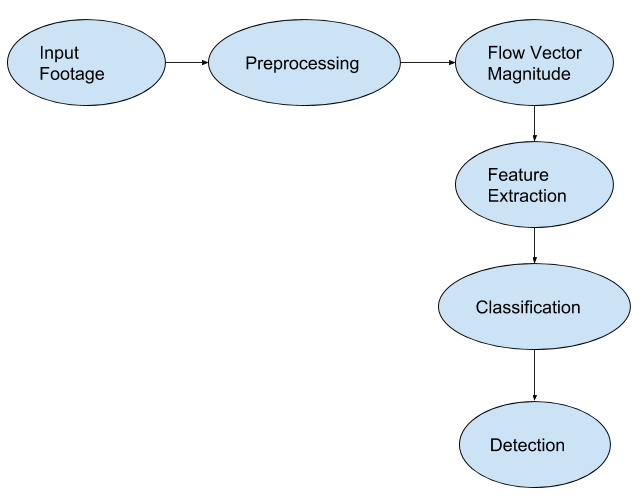
\includegraphics[scale = 0.4]{system_design.png}
\caption{System Design}
\end{figure}

\section{Implementation of Proposed Solution}
\subsection{Input Footage}
For training of the classifier input of the footage will be from a fixed dataset. For practical real time implementation footage from externally attached cameras can be used. The resolution of the input footage need not be specific. Generally the resolution of a CCTV footage is of 704 X 480 pixels. This proposed algorithm reduces the height of the video to 100 pixels and width accordingly. This increases the scalability of the algorithm. Even high definition videos can be processed with the proposed algorithm.
\subsection{Preprocessing}
Preprocessing the input data is very important part of the algorithm. Optical flow algorithm will take at least one minute to calculate optical flow of a high definition image. So as to constraint the processing to real time preprocessing must done. As mentioned earlier any image is being resized to 100 pixel height and respective width accordingly. Preprocessing is done in a way such that the aspect ratio of the video is not disturbed.
\subsection{Flow Vector Magnitude}
For each pixel in the video has some velocity corresponding to it, along x direction and y direction. The Flow Vector Magnitude is nothing but the magnitudes of these velocities. Computing Flow Vector Magnitude is computationally heavy, this is the most time taking part of the proposed algorithm. Since we are reducing the size of frames considerably, this is computation is quick enough to cope us with real time violence detection.
\subsection{Feature Extraction}
Feature extraction is based on the computation of ViF (Violence Flow Descriptors). These descriptors are quantised values of the above generated Flow Vector Magnitudes. After ViF is generated a histogram is built which will assign different ViF values to corresponding bins in the range of (0 to 1.0) with the intervals of 0.05, i.e 20 bins.
\subsection{Classification}
After the features have been extracted, classification can done with the help of a simple Linear SVM. So as to further increase the accuracy of the algorithm , SVM with AdaBoost can be used. For our project a trained neural net has been used since it is providing a better accuracy.
\subsection{Detection}
Detection in a video footage is the final output of the proposed algorithm. It is taking place with the help classifier model that is being trained in the above step. According to the base paper, a sequence of 10 frames i.e on an average two-fifth of a second is enough to detect violence in a footage. Detection may be further improved continuous learning in real-time also.



